
\section{Notion de champ de vecteurs associée à une EDO}
\subsection{Généralités et définitions}
Les modèles continus de la dynamique de populations sont des \underline{problèmes de Cauchy} pour les EDO.
\begin{align*}
    \text{(EDO)} \begin{cases}
        y'(x) = f(t, y(t)) &\qquad t \in ]0, \pi[ \\
        y(0) = y_0  
    \end{cases}
\end{align*}
Où \begin{align*}
    y: [0, \pi] &\longrightarrow \R \\
    t &\longmapsto y(t) 
.\end{align*}
\begin{align*}
    f: ]0, \pi[ \times \R &\longrightarrow\R\\
    (t, x) &\longmapsto f(t, x) 
.\end{align*}

\begin{itemize}
    \item Si l'on sait résoudre analytiquement l'EDO (i.e donner l'expression de $t \mapsto y(y)$) alors c'est terminé car il suffit d'étudier la fonction $t \mapsto y(t)$
    \item Si l'on ne sait pas détérminer la solution analytique, \underline{on peut}:
        \begin{enumerate}
            \item s'assurer de \textbf{l'éxistence} et \textbf{l'unicité} de la solution et de sa \textbf{stabilité} vis à vis des données du problème.
            \item Puis analyser les propriétés qualitatives de cette solution pour simple analyse de $f(t, x)$
                \begin{center}
                    \textbf{C'est ici qu'intervient les champs de vecteurs.} 
                \end{center}
        \end{enumerate}
\end{itemize}
Illustations.
\begin{enumerate}
    \item Prenons le modèle de Malthus
        \[
        \begin{cases}
            N'(t) = r N(t), \quad t \in ]0, \pi[\\
            N(0) = N_0
        \end{cases}
        \] 
        On sait que $N(t) = N_0 e^{rt}$
    \item Voici ce que fait python pour traiter $N$.
        \begin{figure}[H]
            \centering
            \incfig{voici-ce-que-fait-python}
            \caption{Ce que fait python}
            \label{fig:voici-ce-que-fait-python}
        \end{figure}
    \item Traitons les vecteurs tangents à la courbe $t \mapsto N(t)$ aux points  $t_n$, $n=0$ 
    \item Si l'on connaît les valeurs minimals et maximales de la solutions on peut avoir l'allure de la solution.
        \begin{figure}[H]
            \centering
            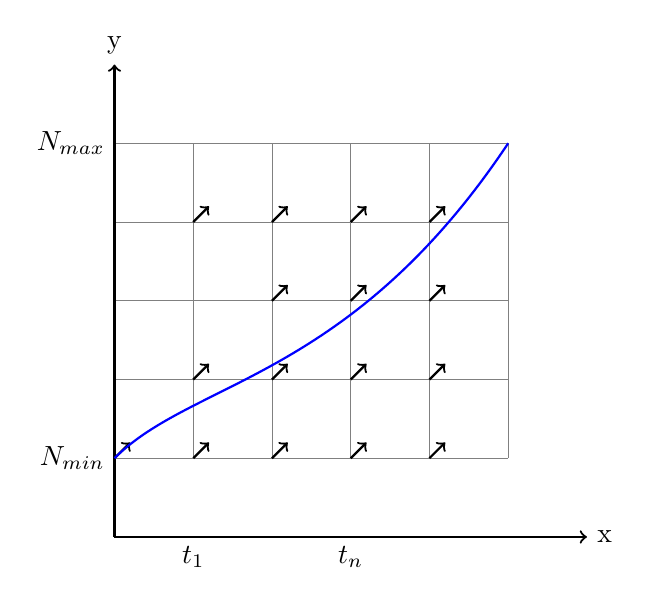
\begin{tikzpicture}
                % Draw the grid
                \draw[step=1cm, gray, very thin] (0,1) grid (5,5);

                % Add axis lines
                \draw[thick,->] (0,0) -- (6,0) node[right] {x};
                \draw[thick,->] (0,0) -- (0,6) node[above] {y};

                \draw[thick,->] (0,1) -- +(0.2, 0.2);
                \draw[thick,->] (1,1) -- +(0.2, 0.2);
                \draw[thick,->] (1,2) -- +(0.2, 0.2);
                \draw[thick,->] (1,4) -- +(0.2, 0.2);
                \draw[thick,->] (2,1) -- +(0.2, 0.2);
                \draw[thick,->] (2,2) -- +(0.2, 0.2);
                \draw[thick,->] (2,3) -- +(0.2, 0.2);
                \draw[thick,->] (2,4) -- +(0.2, 0.2);
                \draw[thick,->] (3,1) -- +(0.2, 0.2);
                \draw[thick,->] (3,2) -- +(0.2, 0.2);
                \draw[thick,->] (3,3) -- +(0.2, 0.2);
                \draw[thick,->] (3,4) -- +(0.2, 0.2);
                \draw[thick,->] (4,1) -- +(0.2, 0.2);
                \draw[thick,->] (4,2) -- +(0.2, 0.2);
                \draw[thick,->] (4,3) -- +(0.2, 0.2);
                \draw[thick,->] (4,4) -- +(0.2, 0.2);
                \node[left] (_) at (0,1){$N_{min}$};
                \node[left] (_) at (0,5){$N_{max}$};
                \draw[thick, blue] (0, 1) .. controls (1,2) and (3,2) .. (5, 5);
                \node[below] (_) at (1, 0){$t_1$};
                \node[below] (_) at (3, 0){$t_n$};
            \end{tikzpicture}  
            \caption{Une courbe sur des champs de vecteurs}
        \end{figure}
\end{enumerate}
Analysons ce que represente le vecteurs tangent:
\begin{itemize}
    \item pour une courbe $y = g(x)$
    \item python et tout autre logiciel procède ainsi
\end{itemize}
\begin{figure}[H]
    \centering
    \incfig{analysons-ce-que-represente-vecteur}
    \caption{Ce que represente vecteur}
    \label{fig:analysons-ce-que-represente-vecteur}
\end{figure}
Le vecteur tangent à la courbe:
\begin{align*}
    \vec{v} = (1, g'(x)) = (1, \frac{dy}{dx}) = (1, \frac{\frac{dy}{dt}}{\frac{dy}{dt}})\\
= \frac{1}{\frac{dy}{dt}}(\frac{dx}{dt}, \frac{dy}{dt}) = \underset{\in \R}{ \frac{1}{\dot{x}(t)} }\underbrace{(\dot{x}(t), \dot{y}(t))}_{\text{vecteur tangent}}
\end{align*}
\[
    \vec{v} = (\dot{x}(t), \dot{y}(t))
\] 
Càd $\vec{v}$ est le vecteur vitesse au points  $M(x(t), y(t))$ a la courbe parametrée  $t \mapsto \begin{cases}
    x(t) = t\\
    y(t) = g(t)
\end{cases}$. On a le résultat.
\begin{prop}
    \begin{align*}
        &\left(\text{y obtient solution de l'EDO } y'(t)=f(t, y(t)) \right) \\
        &\rotatebox{90}{$\iff$}\\ 
        &(\text{vecteur vitesse de la courbe parametrée } t \mapsto (x(t), y(t)) \text{ au point } M(t_0) = (t_0, y(t_0))\\ 
        &\text{ si le vecteur } (1, f(t_0, y(t_0))))  
    \end{align*}
\end{prop}
\begin{prop}
   \begin{align*}
       V: \R^2 &\longrightarrow \R^2 \\
       (t, y) &\longmapsto V((t, y))
   .\end{align*} 
   \[
       \text{(si le champ de vecteur associé à l'EDO } y'(t) = f(t, y(t)) \text{)} \iff V(t, y) = (1, f(t, y))
   \] 
\end{prop}
\subsection{Dessins de champs de vecteurs}
\textbf{\large Principe:}\\
À chaque points $P = (p_x, p_y)$ on trace le vecteur  $\epsilon V(P)$ où  $\epsilon$ est une constance positive choisi pour écrire les vecteurs trop longs.\\
Avec python on écrit \textit{quiver($P_x, P_y, V_x, V_y,$ angles='xy')}
RQ 1: Cette fonction est vectorielle, i.e $P_x, P_y, V_x, V_y,$ sont des numpy array de taille  $n$.
RQ 2: On peut ajouter un paramètre pour controles la longeur des vecteurs:
 \begin{center}
   plt.quiver($P_x, P_y, V_x, V_y$, angles='xy', sacle=$1$) 
\end{center}
Par conséquent, il faut normaliser les vecteurs (i.e le champ de vecteur)
\begin{eg}
   Champ de vecteur du modèle de Verhulst:
   \begin{lstlisting}
       
       def f(t, y):
         return r * y * (1 - y/k)
     \end{lstlisting}
    la grille:

   \begin{lstlisting}
       lt = np.linspace(tmin, tmax, N+1)
       ly = np.linspace(ymin, ymax, M+1)
       T, Y = np.meshgrid(lx, ly)
   \end{lstlisting}
    Construire les vecteurs:

    \begin{lstlisting}
        
       Y = 1 + 0 * T
       V = f(T, Y)
       norm = np.sqrt(U*U + V*V)
        U = U/norm
        V = V/norm
    \end{lstlisting}
    On place les points:
    \begin{lstlisting}
       plt.scatter(T, Y, marker='+', alpha = 0.5)
\end{lstlisting}
    On place les vecteurs
    \begin{lstlisting}
       plt.quiver(T, Y, U, V, angles='xy', scale=N)
\end{lstlisting}
\end{eg}
\subsection{Recherche de solution approchée de modèles sous python}
On cherche une solution approchée de 
\[
\begin{cases}
    y'(t) = f(t, y(t)) \quad t \in ]t_0, t_0 + T[\\
    y(t_0) = y_0
\end{cases}
\] avec python. Pour cela il suffit de dire \textbf{en quels points} on veut cette solution.\\
On se donne:
\begin{itemize}
    \item une liste des instants [$t_0, t_1, \ldots, t_N$]
    \item $t_0, y_0$
    \item Puis, on appelle la fonction \underline{odeint} du module \underline{scipy.integrate} de python.
    \item On obtient une liste [$y_0, y_1, \ldots, y_N$]
\end{itemize}
\begin{eg}
   Cas du modèle du Verhulst 
   \begin{itemize}
       \item EDO:
           \begin{lstlisting}
              def f(t, y):
                return \ldots
           \end{lstlisting}
       \item Instants
           \begin{lstlisting}
              t0, tf = a, b 
              N = 100
              t = np.linspace(t0, tf, N)
           \end{lstlisting}
       \item On appelle odeint
           \begin{lstlisting}
              from scipy.integrate import odeint
              yapp = odeint(f, t, y), rtol=None, atol=None, tfloat=False)
              plt.plot(t, yapp, \ldots)
           \end{lstlisting}
   \end{itemize}
\end{eg}
\section{Modèle de prédateur prose (lotka-voltena (1931))}
$H(t)$: population de sardins\\
$P(t)$: pupulation de reguins
 \[
     \frac{H'(t)}{H(t)} = \text{taux de variation de sardins} = \underbrace{a}_{\text{taux de croissance}} - \underbrace{b P(t)}_{\text{taux de mortalité}}
\] 
\[
    \frac{P'(t)}{P(t)} = \text{taux d'arrivé des requetes} = \underbrace{-c}_{\text{taux de décès}} + \underbrace{d H(t)}_{\text{taux de croissance}}
\] 
D'où le modèle:
\[
\begin{cases}
    H'(t) = H(t)(a - b P(t)) \quad t>0\\
    P'(t) = P(t)(-c + d H(t))\\
    H(0) = H_0, \quad P(0) = P_0
\end{cases}
\] 
Si l'on désigne par $p\ge 0$ la proportion des requêtes en sardines pêchés
\[
\begin{cases}
    H'(t) = H(t)(a - p - b P(t)) \quad t > 0\\
    P'(t) = P(t)(-c - p - d H(t))\\
    H(0) = H_0\\
    P(0) = P_0
\end{cases}
\] 
